\chapter{Implementation}\label{chapter:implementation}
Our driver implementation takes architectural inspiration from the driver implemented in Redox, as well as notes from SPDK, additionally many utility functions are adapted from those in \texttt{ixy.rs} \cite{ixy.rs}. All NVMe commands and directives are implemented based off of Revision 1.4 of the NVMe Specification \cite{nvme-spec}.

\section{User Space Drivers}
Like SPDK, our driver runs entirely in user space, and implements zero-copy I/O operations, as well as a poll-based architecture; SPDK\footnote{\url{https://spdk.io}} being the de-facto standard for NVMe devices in high throughput environments. To write a user space driver, we make use of all the concepts explained in \autoref{chapter:basics}. The driver is able to access the device after memory mapping device files from user space, which offers more flexibility, simplicity, and stability over kernel drivers, with access to debugging tools and overall less restrictions the development of user space drivers is much easier and the ability to use any programming language is also guaranteed. User space drivers are also less likely to cause system crashes or kernel panics due to bugs; faults in user space can often be handled gracefully, improving overall system stability. By avoiding context switches, these drivers are able to reduce overall latency and increase throughput.

Given these advantages, we chose to develop a user space NVMe driver rather than kernel space.

\section{Memory-Mapped I/O}\label{section:MMIO}

\autoref{lst:mmap} shows how to implement memory-mapping a PCIe resource in Rust. In this example, we open the \texttt{resource0} file with read and write access and pass the file descriptor and its length to \texttt{libc::map}. As \texttt{libc::mmap} directly calls \texttt{mmap(2)}, the function call is wrapped in an \texttt{unsafe} block. The BARs are mapped as shared memory, so changes to the mapped memory are also written back to the file and vice-versa. If the function returns a null pointer or the length of the file is 0, we return an error, otherwise the pointer and the length of the file are returned as a pair.

\begin{lstlisting}[float, language=Rust,label=lst:mmap,caption=Memory mapping a PCIe resource in Rust]
pub fn pci_map_resource(pci_addr: &str) -> Result<(*mut u8, usize), Error> {
    let path = format!("sys/bus/pci/devices/{}/resource0", pci_addr);

    let file = fs::OpenOptions::new().read(true).write(true).open(&path)?;
    let len = fs::metadata(&path)?.len() as usize;

    let ptr = unsafe {
        libc::mmap(
            ptr::null_mut(),
            len,
            libc::PROT_READ | libc::PROT_WRITE,
            libc::MAP_SHARED,
            file.as_raw_fd(),
            0,
        ) as *mut u8
    };

    if ptr.is_null() || len == 0 {
        Err("pci mapping failed".into())
    } else {
        Ok((ptr, len))
    }
}
\end{lstlisting}

\section{Direct Memory Access}
To enable the transfer of data between the host system and NVMe device we make use of DMA. We initialise DMA memory for all Submission and Completion Queues, as well as buffers where the device can read from and write to.
As PCIe devices access memory via physical addresses independently of the CPU, we require the buffers we use for DMA to stay in main memory. We can use \texttt{mlock(2)} to guarantee a memory page is locked in main memory, however the mapping is not static for \qty{4}{\kibi\byte} pages, the standard page size on Linux. Instead, we make use of \qty{2}{\mebi\byte} huge pages for this, where the physical addresses are pinned in Linux \cite{user_space_net}.
Enabling the usage of huge pages on the operating system is done with the shell script \texttt{setup-hugetlbfs.sh} which creates a mount point for huge pages and writes a number of huge pages to \texttt{sysfs} files. Now we can allocate memory by creating the file in the newly mounted directory and then memory map the file with \texttt{mmap(2)} and lock it in memory with \texttt{mlock(2)} by using the appropriate bindings in the \texttt{libc} crate. We then derive the physical memory address of the page through \texttt{/proc/self/pagemap}.

\begin{figure}
  \centering
    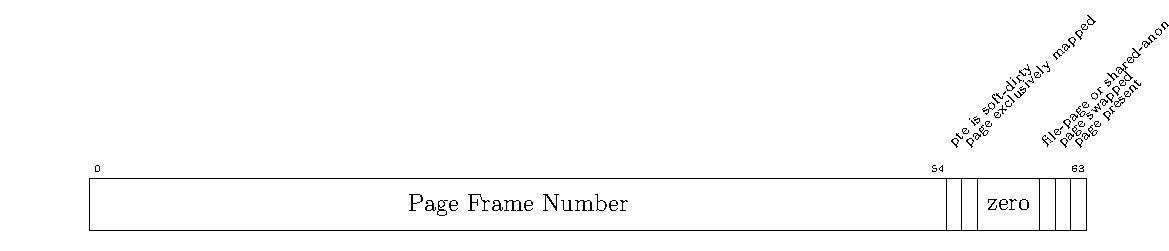
\includegraphics[width=\textwidth]{figures/pagemap}
    \caption{Fields of a pagemap entry when the page is present in main memory}
    \label{fig:pagemap}
\end{figure}

The pagemap contains one 64 bit value for each virtual page; our hugepage is in main memory, so the pagemap entry is structured as depicted \autoref{fig:pagemap}. Finding the relative index of the page is done by taking the virtual address of it and dividing it by the the page size, which we use to locate the corresponding pagemap entry. Constructing the physical address from the pagemap entry and virtual address is done by taking the Page Frame Number (Bits 0-54), multiplying that by the page size to get the physical address of the page, to which we add (virtual address$\mod$page size), the offset within the physical page. For \qty{2}{\mebi\byte} pages this offset is 0. \autoref{lst:virt_phys} shows how this is done in Rust.

One of the reasons the driver runs as root is due to requiring \texttt{CAP\_SYS\_ADMIN} to be able to read the Page Frame Numbers since the Rowhammer vulnerability exploit, i.e. since Linux 4.0.

\begin{lstlisting}[float, language=Rust, label=lst:virt_phys,caption=Translating a virtual address to its physical address]
fn virt_to_phys(addr: usize) -> Result<usize, Error> {
    let pagesize = unsafe { libc::sysconf(libc::_SC_PAGESIZE) } as usize;

    let mut file = fs::OpenOptions::new()
        .read(true)
        .open("/proc/self/pagemap")?;

    file.seek(io::SeekFrom::Start(
        (addr / pagesize * mem::size_of::<usize>()) as u64,
    ))?;

    let mut buffer = [0_u8; mem::size_of::<usize>()];
    file.read_exact(&mut buffer)?;

    let phys = unsafe {
      mem::transmute::<[u8; mem::size_of::<usize>()], usize>(buffer)
    };
    Ok((phys & 0x007F_FFFF_FFFF_FFFF) * pagesize + addr % pagesize)
}
\end{lstlisting}

For DMA we define the struct \texttt{Dma<T>}, with which we can allocate a memory-mapped huge page, encapsulating its virtual address type \texttt{*T} and physical address. We also define the trait \texttt{DmaSlice} which allows us to iterate over chunks of the DMA memory, as well use a subsection of the memory via slicing. This trait is used for zero-copy I/O operations.

\section{Architecture}
Our overall goal was to design a light-weight driver where external dependencies are kept to a minimum. As such, we only require the crates \texttt{libc} for bindings to C library functions, and \texttt{byteorder} for reading different sized integers and to avoid unnecessary unsafe code from working with raw bytes.

The entry point to accessing an NVMe device on our driver is the \texttt{NvmeDevice} struct (\ref{lst:nvmedevice}). Like in Redox, we designed this struct to be able to handle all NVMe operations, i.e. Administrative and I/O capabilities, however as we haven't implemented \texttt{async}, these requests currently operate synchronously. To enable multithreaded I/O processing, we have defined \texttt{NvmeQueuePair}, so like SPDK each thread can have its own queue pair to handle reading and writing, without needing locking access to a single instance of \texttt{NvmeDevice}. With the queue pair submissions and completions can be handled independently of another.

\begin{lstlisting}[float, language=Rust,label=lst:nvmedevice,caption=NvmeDevice struct definition]
pub struct NvmeDevice {
    pci_addr: String,
    addr: *mut u8, // BAR address
    len: usize, // BAR length
    dstrd: u16, // Doorbell stride
    admin_sq: NvmeSubQueue, // Queues
    admin_cq: NvmeCompQueue,
    pub io_sq: NvmeSubQueue,
    pub io_cq: NvmeCompQueue,
    buffer: Dma<u8>,           // 2MiB of buffer
    prp_list: Dma<[u64; 512]>, // PRP list
    pub namespaces: HashMap<u32, NvmeNamespace>,
    q_id: u16,
}
\end{lstlisting}

\section{Driver initialisation}
In this section, we will go over the initialisation process of the driver, looking what happens within the function \texttt{init()} in \texttt{lib.rs} and the functions it calls; \texttt{init()} returns an instance of \texttt{NvmeDevice}, if nothing goes wrong. The struct is the driver for a single NVMe drive, and can handle admin and I/O requests.

Before any configuration and initialisation is done, we check if the PCIe device has the class id \texttt{0x0108}: \texttt{0x01} for mass storage device, \texttt{0x08} the NVMe subclass.
We then unbind the kernel driver from the NVMe device by writing the PCIe address of the device to the \texttt{unbind} file in \texttt{sysfs}. This is then followed by enabling the bus master and disabling interrupts by setting the appropriate bits in the PCI command register, thus enabling DMA and disabling interrupts entirely, as our driver is poll-based. At this point, we also initialise all the relevant structs required for the driver e.g., admin and I/O queues.

The BARs of the NVMe device is then mapped into main memory, as described in \autoref{section:MMIO}. We then follow the initialisation procedure described in the NVMe specification: first, we disable the controller by setting the \texttt{EN} (enable) bit to 0 in the \texttt{CC} (Controller Configuration) register. We wait for the \texttt{ready} bit in the \texttt{CSTS} register to be set to 0, after which we can configure the controller. Configuring the controller involves setting register values to those we require, for example the attributes of the Admin Queues, as well as command entries. All relevant offsets for the registers are stored in the enum \texttt{NvmeRegs32} and \texttt{NvmeRegs64}. The controller is then enabled by setting the \texttt{EN} bit to 1, and we wait for the \texttt{CSTS} register to be set to 1. Now the NVMe controller is ready to process admin submissions.

Although we use unsafe functions to access the BARs of the NVMe device, with an assertion guard, we can make sure that all accesses to the registers are not out of bound (see \autoref{lst:reg32}).

% accessing register be like
\begin{lstlisting}[float, language=Rust, label=lst:reg32,caption=Writing to a 32 bit register]
fn set_reg32(&self, reg: u32, value: u32) {
    assert!(reg as usize <= self.len - 4, "memory access out of bounds");
    unsafe {
      std::ptr::write_volatile(
        (self.addr as usize + reg as usize) as *mut u32, value
      );
    }
}
\end{lstlisting}

After this, we request an I/O completion queue, followed by a request for an I/O submission queue, so the \texttt{NvmeDevice} can do I/O operations. Finally, we identify the namespaces, storing these in a \texttt{HashMap} in the \texttt{NvmeDevice}.

\section{I/O Operations}\label{subsection:io}
As all commands are processed through submission and completion queues, we have defined the structs \texttt{NvmeSubQueue}, and \texttt{NvmeCompQueue}, which store a \texttt{NvmeCommand} array, and \texttt{NvmeCompletion} array on a huge page, respectively. The submission entry being 64 bytes in size means that at most 1024 entries fit on a \qty{2}{\mebi\byte} huge page; for simplicity, we have not implemented queues which span over multiple pages. Thus the maximum number of outstanding submissions we currently support is 1023.

The struct \texttt{NvmeDevice} is able to run as the driver itself, handling admin and I/O commands and also polling their completions, thus it exposes I/O operations with the methods \texttt{read()}, \texttt{write()}, \texttt{read\_copied()}, \texttt{write\_copied()}, as well as \texttt{read\_batched()} and \texttt{write\_batched()}. The initial two methods are zero-copy, taking a reference to a struct which implements the trait \texttt{DmaSlice} as the source buffer for writes and destination for reads, allowing us to iterate over the object in 8096 byte chunks. Currently we only iterate over 8096 bytes, as that is the maximum length we can pass to the NVMe command without the use of PRP lists. If we were to use PRP lists, each request would require constructing a PRP list on a DMA-able buffer.

The latter four methods take a \texttt{u8} slice, which gets copied into the \texttt{NvmeDevice}'s DMA buffer for writes, and copied from for reads. In \texttt{read\_copied()} and \texttt{write\_copied()} we iterate over \qty{512}{\kibi\byte} chunks. \texttt{read\_batched()} and \texttt{write\_batched()} both take a parameter specifying the batch size of the operation. Here we also iterate over \qty{512}{\kibi\byte} chunks, but instead of a single submission request for each chunk, we split it into multiple submissions which get simultaneously added to the queue and polled for. As NVMe SSDs can process multiple submissions at once, batching generally leads to higher throughput, similarly to how increasing queue depth improves performance.

Submitting I/O requeusts is also possible with \texttt{NvmeQueuePair}, using the method \texttt{submit\_io()}, which like \texttt{read()} and \texttt{write()} receives a reference to a \texttt{impl DmaSlice}. This method iterates over \qty{8096}{\byte} as well and returns the number of requests added to the submission queue. It is the user's responsibility to poll for the completion of a command with \texttt{complete\_io()}, which takes the number of submissions to poll for and returns an \texttt{Option<NvmeCompletion>}.

Aside from the data buffer, the user also passed the logical block address (LBA) for the I/O operation. The length of data written is derived from the length of the buffer.
